\documentclass{article}

% Set page size and margins
% Replace `letterpaper' with`a4paper' for UK/EU standard size
\usepackage[letterpaper,top=2cm,bottom=2cm,left=3cm,right=3cm,marginparwidth=1.75cm]{geometry}

% Useful packages
\usepackage{amsmath}
\usepackage{graphicx}
\usepackage[colorlinks=true, allcolors=blue]{hyperref}

\title{Problem Set 5 - ECON 5253}
\author{Thomas Mondry}

\begin{document}
\maketitle

\section{Web scraping -- J! Archive}

For this problem, I wanted to try out manual web scraping from the suboptimally-formatted J! Archive website to see whether this would be a feasible approach to data acquisition for my final project. The site is flashy and clearly tailored toward the experience of someone viewing the games one at a time in browser, with correct responses \& some other information usually only displayed on mouseover. While the way \texttt{rvest} parses the tables is hard to read and somewhat unpredictable (see Figure 1), it is consistent (from what I can tell) among different rounds from different games, meaning it is possible to programmatically transform the data from many games into a readable format. I gave this a shot here, deciding that the best approach would be to start entirely from scratch with an empty data frame of relevant information, which I then populated one row at a time by looking in the right places in the raw data. One trick I found was that while the absolute location of the information of interest for each clue within the entire table doesn't follow a consistent pattern, its position relative to a respective \texttt{NA} cell is consistent, so the location of the relevant information can easily be obtained after these \texttt{NA} cells are located.

\begin{figure}[h]
	\centering
	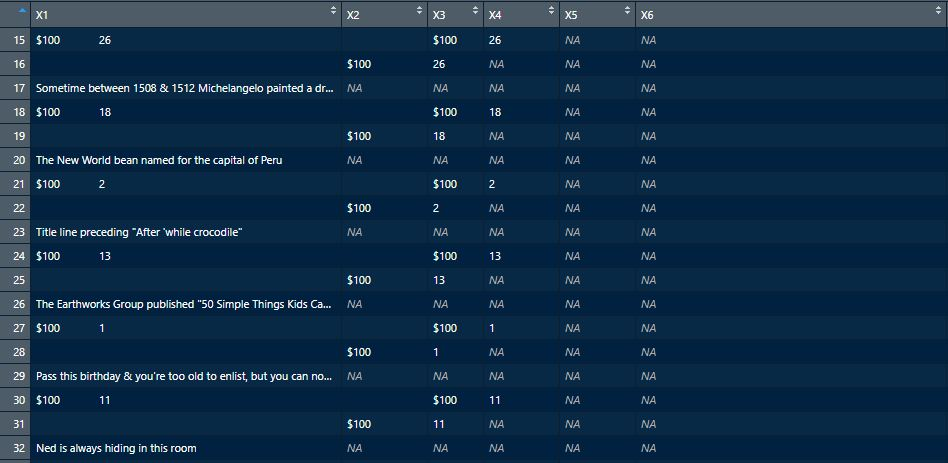
\includegraphics[width=\textwidth]{screenshot_raw.jpg}
	\caption{Part of the raw table of clues, as parsed by \texttt{rvest}}
\end{figure}

The end results here were a table of clue-level information for one round of one game (Figure 2); and, more importantly, a reproducible \& sufficiently efficient process for scraping the data from two different URLs, parsing the correct elements into an R data frame, and transforming the raw data into a usable format. I expect that this process can easily be wrapped into a function which takes the ID of the game on the archive -- fortunately, the URLs on the site appear to be straightforward and consistent -- and returns complete tables of each clue from each game. Since the data contained on the site encompasses most of the quantifiable information about a game (with the exception of buzzer times and other information which is very difficult to obtain), I believe my process will be sufficient for tackling any data-driven question about the game which I may want to investigate for my final project, although there are a few more pieces of information which I'd like to integrate into the process.

\begin{figure}[t]
	\centering
	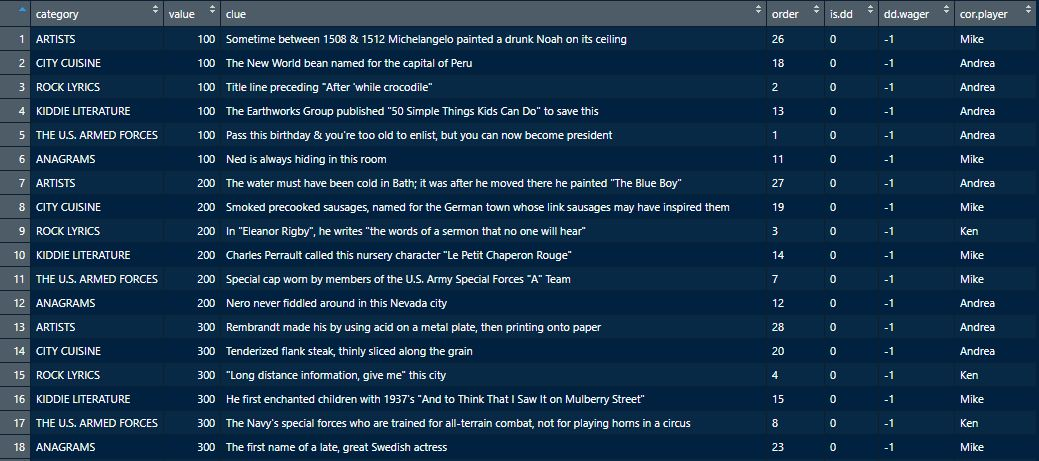
\includegraphics[width=\textwidth]{screenshot_clean.jpg}
	\caption{Part of the cleaned data table for the Jeopardy round which aired 05/23/1991}
\end{figure}

\section{API -- Spotify data}

For this problem, I pulled data from the Spotify API using the \texttt{spotifyr} package. I decided to take advantage of the audio features which the Spotify API provides in order to quantitatively compare several recordings of the same piece of music -- Faur\'e's \textit{Requiem}. I used the API to find 10 popular albums that consist solely of the \textit{Requiem}, then obtained audio features for each track of each album, and finally averaged these audio features for each album in order to compare the recordings quantitatively.

\begin{figure}[h]
	\centering
	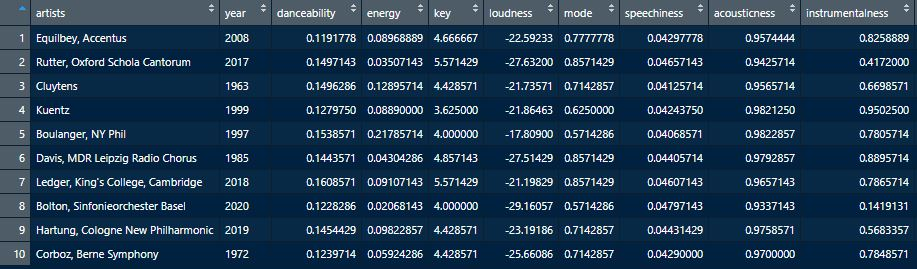
\includegraphics[width=\textwidth]{screenshot_faure.jpg}
	\caption{Table with a few features for some recordings of the Faur\'e \textit{Requiem}}
\end{figure}

Glancing at the results, there doesn't appear to be a lot of major variation in the features. This is to be expected -- everyone is fundamentally performing the same music. A couple of notes:

\begin{itemize}
	
\item It appears at first that the Nadia Boulanger/NY Phil recording is a big outlier, as its loudness and energy scores are much higher than the other recordings; however, a quick listen reveals that this is likely because it is a live recording, and a very old one at that (the performance is from 1962), so recording technology didn't allow for the removal of audience coughs and other ambient noises.

\item For some reason, the Bolton/Sinfonieorchester Basel recording has a surprisingly low instrumentalness score of 0.142, where most of the others are in the 0.6-0.9 range. It sounds like this recording was made on period string instruments, which have a slightly "harsher" sound -- maybe the algorithm that generates the audio features interpreted this sound as electronic, but it doesn't seem like the difference should be so pronounced.

\end{itemize}

\end{document}